\documentclass{aa}
% \documentclass[referee]{aa}
\usepackage[varg]{txfonts}
\usepackage[separate-uncertainty=true]{siunitx}
\usepackage[version=3]{mhchem}
\usepackage[colorlinks, linkcolor=black, citecolor=blue]{hyperref}

\sisetup{range-units = brackets}

\def\eps{\varepsilon}
\def\aap{A\&A}
\def\eprint{e-prints}
\def\apj{ApJ}
\def\apjs{ApJS}
\def\apjl{ApJL}
\def\mnras{MNRAS}
\def\aj{AJ}
\def\nat{Nature}
\def\aaps{A\&A Supp.}
\def\prd{Phys. Rev. D}
\def\prl{Phys. Rev. Lett.}
\def\araa{ARA\&A}

\bibpunct{(}{)}{;}{a}{}{,}


\begin{document}


\title{High resolution near-IR spectroscopy of Arcturus and 10 Leo}
\subtitle{Refining a near-IR iron line list}


\author{ D.~T.~Andreasen\inst{1,2}
    \and S.~G.~Sousa\inst{1}
    \and E.~Delgado Mena\inst{1}
    \and N.~C.~Santos\inst{1,2}
    \and T.~Lebzelter\inst{3}
    \and A.~Mucciarelli\inst{4,5}
    \and J.J.~Neal\inst{1,2}}


\institute{
  Instituto de Astrof\'isica e Ci\^encias do Espa\c{c}o, Universidade do Porto,
    CAUP, Rua das Estrelas, 4150-762 Porto, Portugal,
    \email{daniel.andreasen@astro.up.pt}
  \and
    Departamento de F\'isica e Astronomia, Faculdade de Ci\^encias, Universidade
    do Porto, Rua Campo Alegre, 4169-007 Porto, Portugal
  \and
    Institute for Astrophysics, University of Vienna, T\"urkenschanzstrasse 17,
    1180 Vienna, Austria
  \and
    Dipartimento di Fisica e Astronomia, Universita' degli Studi di Bologna, Viale
    Berti Pichat, 6/2, 40126, Bologna, Italy
  \and
    INAF - Osservatorio Astronomico di Bologna, Via Ranzani 1, 40127, Bologna,
    Italy
}





\date{Received ...; accepted ...}

\abstract
% Context
{Reliable stellar atmospheric parameters for FGK stars have been {\bf commonly} obtained from
methods that rely on high resolution and high S/N optical spectroscopy. The advent of a new
generation of high resolution {\bf ($R>50\,000$)} near-IR spectrographs opens the possibility of
using classic spectroscopic methods with high resolution and high S/N in the NIR spectral window.}
% Aims
{We aim to {\bf refine a NIR iron line list for determination of stellar atmospheric parameters. For
verification we derive parameters of two K giant stars, Arcturus and 10 Leo.}}
% Methods
{Our spectroscopic analysis is based on the iron excitation and ionization balance done in LTE and a
line list of \ion{Fe}{I} and \ion{Fe}{II} lines in the NIR domain. The line list is being refined
from our previous study, allowing us to obtain more reliable parameters.}
% Results
{{\bf We present an updated line list for the derivation of stellar parameters in the NIR that has
allowed us to successfully} obtain parameters for two K giants in agreement with average literature
values adopted.}
% Conclusions
{With these results we are now extending our previous line list towards cooler stars, thus allowing
us to explore the M dwarf stars in the future. {\bf The improvement of the derivation of stellar
parameters for M dwarfs is very important for the study of the Galactic Chemical Evolution and
crucial for the characterisation of Earth-like planets, expected to be very common around these kind
of stars.}}



\keywords{data reduction: high resolution spectra --
          stars individual: Arcturus --
          stars individual: 10 Leo}
\maketitle



\section{Introduction}
\label{sec:introduction}

{\bf
The study of stellar atmospheric parameters have always been important in astronomy. These
parameters consists of e.g. the effective temperature, the surface gravity, the chemical composition
of the stellar atmosphere, and the overall metallicity (where $[\ion{Fe}/\ion{H}]$ is often used as
a proxy). These can be derived with many different methods such as, but not limited to, the infrared
flux method (IRFM) \citep{Blackwell1977}, temperature-metallicity-colour correlations \citep[see
e.g.][]{Ramirez2005b}, asteroseismology \citep[see][for a classic example]{Kjeldsen1995}, and
different spectroscopic approaches such as synthetic fitting \citep[see
e.g.][]{Onehag2012,Tsantaki2017} and curve-of-growth analysis.

Not all the methods provide the same information, e.g. can asteroseismology not derive
$T_\mathrm{eff}$ but is in turn dependent on this parameter. On the other hand it is also well known
that the surface gravities provided by asteroseismology are more reliable than those from
spectroscopy \citep[see e.g. the discussion by][]{Mortier2014}.

The derivation of stellar atmospheric parameters can be used to benchmark stellar evolutionary
models, the study of different galactic populations and the galactic chemical evolution, and in
recent years to study star-planet correlations. With the advance of high precision instruments, we
have open entire new windows into the study of stellar astrophysics with e.g. the \emph{Kepler} and
\emph{CoRoT} space missions \citep[see e.g.][]{Christensen-Dalsgaard2010,Chaplin2011,Huber2014}, and
spectrographs like HARPS for searching new exoplanets \citep{HARPS} and UVES \citep{UVES}.

In recent years there has been an emphasis on exploring the near-IR (NIR) domain of the spectrum
with high-resolution spectrographs ($R\ge50\,000$). These includes the GIANO spectrograph installed
at \emph{Telescopio Nazionale Galileo} (TNG) is already available \citep{GIANO}, as is the
\emph{infrered doppler instrument} (IRD) installed at the Subaru telescope \citep{IRD} and
\emph{Calar Alto high-Resolution search for M dwarfs with Exoearths with Near-infrared and optical
Échelle Spectrographs} (CARMENES) at the \SI{3.5}{m} telescope at Calar Alto Observatory
\citep{CARMENES}. Two new spectrographs are planned for the near future: 1) The \emph{CRyogenic
InfraRed Echelle Spectrograph Upgrade Project} (CRIRES+) at the \emph{Very Large Telescope} (VLT)
\citep{CRIRESp} with expected first light in 2017, and 2) \emph{un SpectroPolarimètre Infra-Rouge A
Near-InfraRed Spectropolarimeter} (SPIRou) at \emph{The Canada-France-Hawaii Telescope} (CFHT)
\citep{SPIROU1,SPIROU2} with expected first light in 2017 as well. The spectral resolutions for
these spectrographs range between $50\,000$ and $100\,000$.

With the advance of the next generation high resolution NIR spectrographs, we are still preparing
the data analysis of stellar spectra, in particular how to get reliable atmospheric parameters
\citep[see e.g.][]{Onehag2012,Lindgren2016,Andreasen2016,Passegger2016}. The analysis of stellar
spectra is well understood for FGK stars in the optical part of the spectrum, however some work
still needs to be done for the NIR part.

We continue our study to explore the use of the NIR domain to derive stellar parameters for FGK and
M stars using the curve-of-growth analysis with an iron line list, which was initiated in
\citet{Andreasen2016} (referred to as Paper I). Here we analyse the atlas of Arcturus and the
spectrum of 10 Leo. For the analysis we use the iron line list presented in Paper I which is
improved and updated in this work. In Paper I we successfully tested our method on a slightly hotter
star than the Sun, while in this work we aim to test the method on cooler stars. The strength of the
NIR domain over the optical becomes clear when we move towards the cooler stars. Here we see less
continuum depression and line blending due to in particular molecular features which are more
prominent in the optical part for cool stars. Moreover, the coolest stars emit more light in the NIR
domain than the optical, and with the stars with the lowest masses being intrinsically faint, we
thus obtain the majority of the flux here.
}




\section{Stellar spectra}
\label{sec:data}

While the community is currently on the verge to access large amounts of high resolution NIR
spectra, the available spectra at the moment are sparse. We chose to use two stars cooler than the
Sun since we used a star hotter than the Sun (the subgiant HD 20010) in Paper I {\bf as it was one
of the stars with stellar atmospheric parameters closest to that of the Sun, thus making it a good
test at the time}. We will however use all four stars in this work for various reasons. The solar
spectrum will be used for inspecting the line list presented in Paper I. This spectrum was obtained
from the Kitt Peak telescope by \citet{Hinkle1995}. The spectrum of HD 20010 will be reused from
Paper I as well {\bf in order to check that the line list works well for hotter stars after our
modifications}. This spectrum was obtained with the CRIRES spectrograph by \citet{Lebzelter2012} as
part of the CRIRES-POP. HD 20010 will be reanalysed as to confirm the improvement of the refined
line list which will be presented in the section below. The two stars which we have not analysed
before are Arcturus and 10 Leo. These two extra stars will increase the range of spectral type for
the test of the line list, allowing to test cool giant stars with different metallicities regimes.


Arcturus is one of the brightest stars on the Northern hemisphere, and is well
studied \citep[see e.g.][to mention just a
few]{Griffin1967,McWilliam1990,Ramirez2013}, and a benchmark star in
current spectroscopic surveys such as Gaia-ESO \citep{Jofre2014,Smiljanic2014}.
The atlas of Arcturus (acquired at Kitt Peak National Observatory using the FTS
spectrograph at the Mayall telescope by \citet{Hinkle1995a}), covers the
spectral range of interest (YJHK bands). Strong telluric features were
identified with a spectrum from the TAPAS web page \citep{Bertaux2014}. The
atlas also comes with a telluric standard and the ratio of the two spectra in
order to correct for the tellurics. The telluric spectrum from TAPAS is only
used for telluric line identification. We use both the telluric corrected and
non-corrected spectrum.

The spectrum for 10 Leo is made available by the CRIRES-POP team
\citep{Nicholls2017}. 10 Leo is very similar to Arcturus, which is also one
reason this star was the first to be fully reduced by the CRIRES-POP team. The
spectrum is divided into several pieces according to the atmospheric windows in
the NIR: YJ (only together), H, K, L, and M. We use only the first three. Some
small gaps are present in the spectrum due to tellurics that could not be
properly removed, low S/N, bad pixels, etc. Rather than giving an uncertain
interpolation, \citet{Nicholls2017} decided to leave small gaps in the data.
This has very little effect on our line by line analysis, however, due to those
gaps, we were unable to measure one \ion{Fe}{II} line which are generally
important to determine the surface gravity.

The data for the two stars are very similar in terms of S/N (around 300 as
measured by IRAF in a continuum region in the YJ band), resolution
(approximately $100\;000$), and spectral coverage.

A summary of the four stars used can be seen in Table~\ref{tab:stars}. The parameters are obtained
from the PASTEL catalogue \citep{Soubiran2016} which is a compilation of stellar atmospheric
parameters from the literature obtained mostly from high resolution and high S/N spectra. {\bf
Specifically for Arcturus, we use the same parameters as reported in Table 1 in} \citet{Jofre2014}.
{\bf These parameters are a mean from the PASTEL catalogue between 2000 and 2012.} The parameters
are the median values of all measurements for a given star, where the errors reported are the
standard deviation of those values. {\bf This also explains the slightly higher errors than what is
usually possible with a single measurement.} $\xi_\mathrm{micro}$ is estimated using the empirical
relation by \citet{Tsantaki2013} for {\bf HD 20010}, and \citet{Adibekyan2015} for the {\bf 10 Leo.
The first relation by \citet{Tsantaki2013} is only valid for $\log g\ge3.85$, while the other
relation is for giant stars. For Arcturus the value is a mean of the derived microturbulence from
different groups as explained in} \citet{Jofre2014}. This is done for each literature value in the
catalogue. The value presented in the Table here is calculated on the same way as the rest of the
parameters.

\begin{table*}[htb!]
    \caption{Summary of the four stars used in this work. The stellar parameters
             are from the PASTEL catalogue \citep{Soubiran2016} (see text for
             details), except the parameters for the Sun.}
    \label{tab:stars}
    \centering
    \begin{tabular}{lllllll}
      \hline\hline
        Star        & Spectrographs  & Resolution  & $T_\mathrm{eff}$ (K) &  $\log g$ (dex)  &   $\xi_\mathrm{micro}$ (km/s)   & [Fe/H] (dex)      \\
      \hline
        Sun         & FTS            & 600\,000    & $5777$               &  $4.44$          &    $1.00$                       & $ 0.00$          \\
        Arcturus    & FTS            & 100\,000    & $4247 \pm  37$       &  $1.59 \pm 0.04$ &    $1.30 \pm 0.12$              & $-0.54 \pm 0.04$ \\
        HD 20010    & CRIRES         & 100\,000    & $6152 \pm  95$       &  $3.96 \pm 0.11$ &    $1.17 \pm 0.24$              & $-0.27 \pm 0.06$ \\
        10 Leo      & CRIRES         & 100\,000    & $4742 \pm  61$       &  $2.76 \pm 0.17$ &    $1.45 \pm 0.08$              & $-0.03 \pm 0.02$ \\
      \hline
    \end{tabular}
\end{table*}

\section{The line list}

There have been different recent studies compiling line lists for high resolution NIR spectra. For M
dwarfs there is the line list by \citet{Onehag2012,Lindgren2016} {\bf which covers the J band},
which has been tested extensively on CRIRES spectra ($R\sim100\,000$) using the spectral synthesis
method. {\bf Then there is the work by \citet{Shetrone2015} for deriving parameters of giant stars
using the H band in APOGEE spectra.}

Since we wanted to compile an iron line list (i.e. only \ion{Fe}{I} and \ion{Fe}{II}) for FGK, and
possible M dwarf stars, suitable for the EW method, we decided to start from the VALD3 database
\citep{VALD1,VALD2}. This was initially done in Paper I as we prepared a \ion{Fe}{I} and
\ion{Fe}{II} line list in the NIR domain. The atomic data from the lines were in a wavelength region
ranging from \SIrange{10000}{25000}{\AA}, covering the YJHK bands. EWs were measured for all iron
lines with ARES \citep{Sousa2015a}, discarding any line with EW below \SI{5}{m\AA} or above
\SI{200}{m\AA}. The oscillator strengths of the line list were calibrated using the solar spectrum,
and the solar iron abundance from \citet{Gonzalez2000} at 7.47 dex. {\bf We chose this reference for
consistency with our previous works on stellar parameters. Nevertheless, we note that this value is
very similar to other more recent values \citep[e.g.][]{Asplund2009}}. The
abundances of individual iron lines were obtained with the radiative transfer code MOOG
\citep{Sneden1973} assuming LTE and using ATLAS model atmospheres \citep{Kurucz1993}. The line list
was successfully used to derive atmospheric parameters for a late F star, HD20010.


\subsection{Refining the NIR line list}
\label{sec:refining_the_line_list}

In this work we will go one step forward, and test the previous line list for two K type stars.
Before testing the line list from Paper I at cooler effective temperatures with two K stars, it is a
primary goal of this work to refine the line list. This includes identifying recurring outliers
(both from the work done in Paper I and in this work), and lines which we are not able to measure,
e.g. if a line is amidst a forest of telluric lines. {\bf These outliers are easier to find with
three spectra compared to just one.} This refinement is needed, since we experienced {\bf an
over-estimated metallicity of around 0.1 dex for HD 20010 compared to the literature value used in
Paper I.} The errors on all parameters were also quite high compared to what is achievable for
similar quality spectra from the visible. To identify these lines the solar atlas used in Paper I
was revisited {\bf which is not clean of tellurics}. In total 211 out of 295 \ion{Fe}{I} lines and 8
out of 13 \ion{Fe}{II} lines were removed in the process. Most of these were blended lines with
either tellurics or other stellar lines. This procedure leaves us with 84 \ion{Fe}{I} lines and 5
\ion{Fe}{II} lines. These lines should be the best for deploying our technique of determining
atmospheric stellar parameters.

During a second look at the Solar spectrum, the EW of the lines were measured by hand (this had
previously been done automatically with ARES). {\bf This process helped us identifying lines that
was blended. In cases where there is severe line blending, the line was discarded as described
above.} Since we re-measured the EWs, the oscillator strengths, $\log \mathit{gf}$, had to be
re-calibrated again. Here we simply change the $\log \mathit{gf}$ values for the measured line until
the abundance of a given line is equal to that of the Sun, using the same solar atmosphere model as
in Paper I. The mean change in $\log \mathit{gf}$ for common lines is $-0.09 \pm 0.16$. The final
revisited line list with the updated $\log \mathit{gf}$ is presented in Table~\ref{tab:linelist}.

The \ion{Fe}{II} lines are used to determine $\log g$ by imposing ionization
balance with the average \ion{Fe}{I} abundance. However, the low number of
\ion{Fe}{II} lines available is a concern, since the average abundance of
\ion{Fe}{II} is affected more by small number statistics compared to the
numerous \ion{Fe}{I} lines.


\section{Obtaining stellar parameters}
\label{sec:method}

The method used both in Paper I and here is based on the determination of the iron abundances on a
number of lines from their measured EWs. This is done using the radiative transfer code MOOG
\citep{Sneden1973} to determine the iron abundance from the measured EWs. Then, ionization balance
between \ion{Fe}{I} and \ion{Fe}{II} lines, and excitation balance for all \ion{Fe}{I} lines is
imposed, by changing the atmospheric parameters for the model atmosphere \citep[][ATLAS9 is used
here]{Kurucz1993}. While this is a well tested method for getting atmospheric parameters utilising
the optical part of the spectrum, {\bf little work has been done with the EW method in the NIR
domain. Therefore we approach the measurements of the EWs with extra care, thus} the measurements of
EWs are done with both manually (IRAF) and automatically (ARES) as a quality check. For both the
automatically and manually measured EWs, we discard all lines with an EW below $\SI{5}{m}$\AA{} and
above $\SI{150}{m}$\AA{} before continuing the analysis. We decided to be a bit more constrained in
the upper limit for the line strength decreasing it to $\SI{150}{m}$\AA{} to be sure that the
Gaussian fit is a good approximation. Lines outside this range are either too weak to be reliably
measured or saturated and do no longer contain information about the abundance. The entire procedure
of obtaining the stellar parameters is done with the software \texttt{FASMA} \citep{Andreasen2017a}
which does the minimization when imposing ionization end excitation balance.




\section{Results}
\label{sec:results}

{\bf The results for the revisited spectrum of HD 20010, and the two additional K stars are
presented here. We do not present the results for the Sun since the line list is calibrated for this
star\footnote{The solar parameters used were: $T_\mathrm{eff}=\SI{5777}{K}$, $\log g=4.44\,$dex,
$[\ion{Fe}/\ion{H}]=0.00\,$dex, and $\xi_\mathrm{micro}=\SI{1.00}{km/s}$.}.}

\subsection{Revisiting HD 20010}
\label{sec:hd20010}

As a first step we revisit HD 20010 for which we derived atmospheric stellar parameters in Paper I
using the newly revised line list presented in this paper. The results are shown in Table
\ref{tab:results} along with the {\bf results for the two other stars analysed in this work}. We see
better agreement with the average literature values adopted (especially $[\ion{Fe}/\ion{H}]$ and
$\log g$), and smaller errors with the updated results, {\bf although errors are still high compared
to optical typical values}. This suggests that the new line list is more reliable.

\begin{table}[htb!]
    \caption{Results for the three stars with first set of parameters are the
             literature values as presented in Table.~\ref{tab:stars}, second
             set of parameters are results with $\log g$ set to the same value
             during the minimization procedure as found in the literature
             (fixed), and last set of parameters are with all parameters free
             during the minimization procedure.}
    \label{tab:results}
    \centering
    \begin{tabular}{llll}
      \hline\hline
                                    & HD 20010          &  10 Leo           &  Arcturus        \\
      \hline
        Literature                  &                   &                   &                  \\
        $T_\mathrm{eff}$ (lit.)     & $6152 \pm  95$    &  $4741 \pm  60$   & $4247 \pm 37$   \\
        $\log g$ (lit.)             & $3.96 \pm 0.19$   &  $2.76 \pm 0.17$  & $1.59 \pm 0.04$  \\
        $[\ion{Fe}/\ion{H}]$ (lit.) & $-0.27 \pm 0.06$  &  $-0.03 \pm 0.02$ & $-0.54 \pm 0.04$ \\
        $\xi_\mathrm{micro}$ (lit.) & $1.17 \pm 0.24$   &  $1.45 \pm 0.08$  & $1.30 \pm 0.12$  \\
      \hline
        $\log g$ fixed              &                   &                   &                  \\
        $T_\mathrm{eff}$            & $6161 \pm 164$    &  $4761 \pm 118$   & $4357 \pm  74$   \\
        $\log g$                    & 3.96 (fixed)      &  2.76 (fixed)     & 1.59 (fixed)     \\
        $[\ion{Fe}/\ion{H}]$        & $-0.18 \pm 0.11$  &  $ 0.01 \pm 0.07$ & $-0.55 \pm 0.04$ \\
        $\xi_\mathrm{micro}$        & $1.72 \pm 0.44$   &  $1.25 \pm 0.11$  & $1.55 \pm 0.10$  \\
      \hline
        All free                    &                   &                   &                  \\
        $T_\mathrm{eff}$            & $6162 \pm 184$    &  $4805 \pm  98$   & $4439 \pm  62$   \\
        $\log g$                    & $4.08 \pm 0.77$   &  $2.42 \pm 0.61$  & $1.20 \pm 0.20$  \\
        $[\ion{Fe}/\ion{H}]$        & $-0.18 \pm 0.11$  &  $-0.01 \pm 0.07$ & $-0.58 \pm 0.06$ \\
        $\xi_\mathrm{micro}$        & $1.59 \pm 0.49$   &  $1.23 \pm 0.10$  & $1.55 \pm 0.10$  \\
        \hline\hline
    \end{tabular}
\end{table}

The parameters for the three stars are presented in Fig.~\ref{fig:parameters}. We show the
literature values (blue), derived parameters with $\log g$ fixed to the literature value (green),
and derived parameters when $\log g$ is free during the minimization procedure (red points).

\begin{figure}[htpb!]
    \centering
    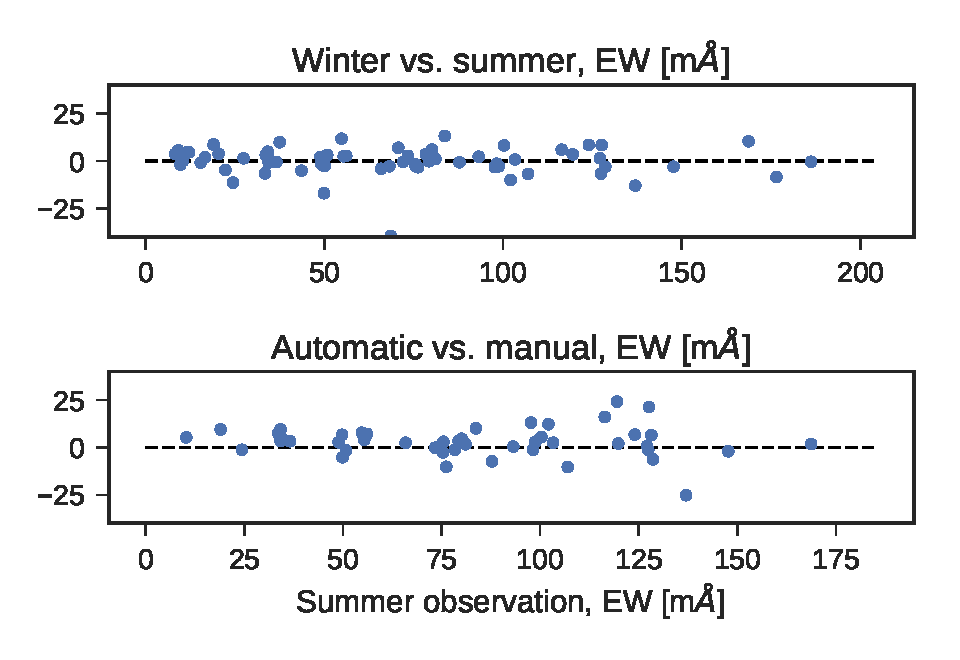
\includegraphics[width=1.0\linewidth]{figures/EWcomp.pdf}
    \caption{Top figure: Difference of the automatic EW measurements between the
             summer observations and winter observations from the Arcturus
             spectra. Bottom figure: Same as above, but with manual measurements
             from ARES (summer) and automatic measurements (summer).}
    \label{fig:EWcomp}
\end{figure}


\subsection{Arcturus}
\label{sec:arcturus}

Arcturus is one of the brightest stars on the night sky with a V magnitude of
-0.05 \citep{Ducati2002}. Hence it is a prime target for testing with the
numerous measurements of the atmospheric parameters as mentioned above.

The atlas consists of both a summer observation set and a winter observation
set. The two data sets have been obtained in order to minimise the effect of
tellurics at different spectral regions. A comparison between the two sets of
measured EWs - both the manual measurements using IRAF and the automatic
measurements using ARES - are shown in Fig.~\ref{fig:EWcomp}. The automatic EW
measurements for the summer set and winter set show excellent agreement
with a {\bf mean difference of 3\%}. This means that the two data sets are very
similar, thus we decided to only manually measure the EWs for one set (summer).
We did, however, measure a few lines from the winter data set to verify the
agreement. Since the EWs are very similar we chose to only derive
parameters of the summer set with EWs measured with ARES.

{\bf Due to the low number of pressure sensitive \ion{Fe}{II} lines we derive} parameters with and
without $\log g$ set to a fixed value (1.59 dex, the average literature value adopted). The
derivation of the parameters followed the procedure presented \citet{Andreasen2017a} with the
minimization routine \texttt{FASMA}. This is similar to the approach done in Paper I. After we
reached convergence using all the iron lines we were able to measure, one outlier above $3\sigma$ in
abundance were removed, and the minimization routine was restarted. This process was done
iteratively until there were no more outliers. The final results are presented in Table
\ref{tab:results} together with mean parameters from the literature.


\begin{figure}[htpb!]
    \centering
    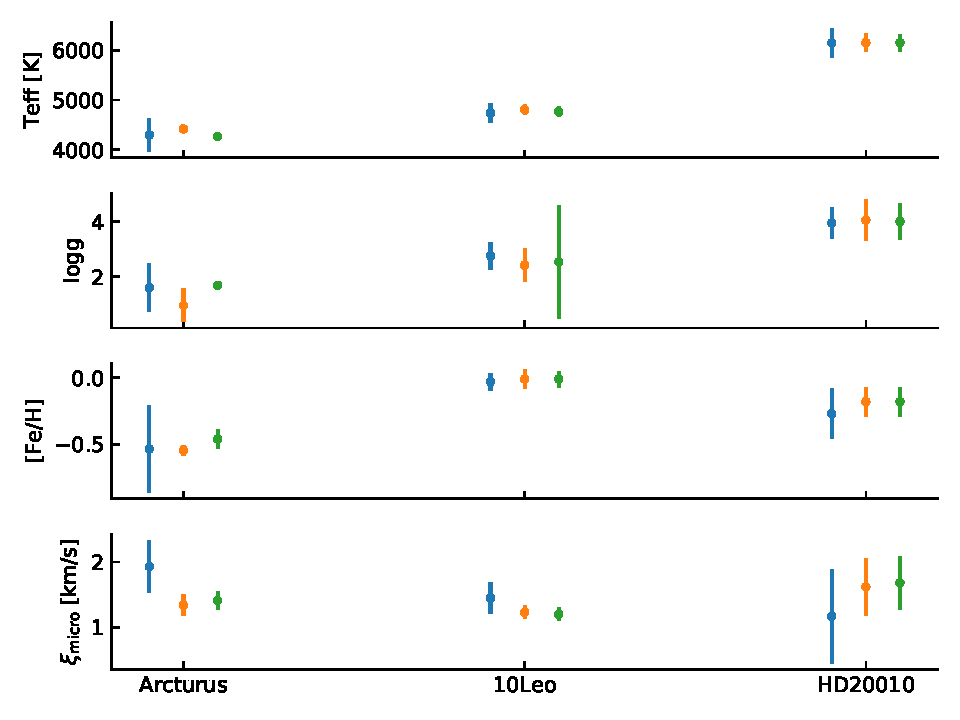
\includegraphics[width=1.0\linewidth]{figures/parameters.pdf}
    \caption{Parameters for Arcturus, 10 Leo, and HD 20010 (revisited in this paper). The blue
             points show the literature values as discussed in the text. The green points are the
             derived values with $\log g$ fixed to the literature value, and the red points show the
             derived parameters when $\log g$ is also derived. {\bf For $T_\mathrm{eff}$ the results
             are shown compared to the literature value to see the difference.}}
    \label{fig:parameters}
\end{figure}

{\bf We derive a $T_\mathrm{eff}$ \SI{100}{K} higher than in the literature with $\log g$ fixed,
which is just within the errorbars of the two measurements. When $\log g$ is derived we see a
\SI{200}{K} difference. This especially shows the effect when $\log g$ is wrong which we here derive
0.4 dex lower than the literature value. The metallicity is derived with rather high precision (0.04
dex) when $\log g$ is fixed and 0.10 dex when it is derived. The value in both cases are well within
the errors of the literature value.}


\subsection{10 Leo}
\label{sec:10Leo}

The approach for determining the atmospheric stellar parameters for 10 Leo is identical to Arcturus,
{\bf although we did not measure the EWs by hand here}. We use ARES on each band (YJ, H, and K-band)
separately. For the small gaps in the spectrum, we simply set the flux to 1, since the spectrum is
already normalised. This will also prevent ARES to identify and measure any lines in these regions.
The EWs from the three regions are combined to one final line list used for the determination of the
parameters. The final results can be seen in Fig.~\ref{fig:parameters} and Table~\ref{tab:results}.

Generally the derived parameters are in excellent agreement with the literature
values listed here.  For $T_\mathrm{eff}$ we were \SI{64}{K} off with $\log
g$ set as a free parameter, well within the errors. The only parameter that show
a discrepancy compared to the literature value is $\xi_\mathrm{micro}$ with a
difference of \SI{0.22}{km/s}, which is at the limit of the errors reported. We
note that this parameter is not reported in the PASTEL database, and this was a
derived parameter from a empirical relation. We were able to derive good $\log
g$ values, although with larger errors compared to the results from the
literature.



\section{Discussion}
\label{sec:discussion}

\subsection{The role of $\log g$}

One of the most difficult atmospheric stellar parameters to get from a spectrum
is the surface gravity. For this we need the lines of pressure sensitive ionized
atoms such as \ion{Fe}{II}. However, they are more sparse than neutral iron,
\ion{Fe}{I}, making the determination more challenging. This is true in the
optical \citep[see e.g. the discussion by][]{Mortier2013c}, and even more in the
NIR (see e.g. Paper I). One solution to this problem is to fix the value of
surface gravity and derive the other parameters. With the parallaxes from e.g.
Gaia \citep{GAIA} we will have access to accurate $\log g$. However, this
requires a priori knowledge of the mass from e.g. isochrones, and
$T_\mathrm{eff}$. By iteratively obtaining the $T_\mathrm{eff}$ from
spectroscopy and the corresponding $\log g$ from the parallaxes, we can obtain
reliable $T_\mathrm{eff}$, $\log g$, and $[\ion{Fe}/\ion{H}]$. Another
approach is to use asteroseismic $\log g$ which are becoming a new standard.
This has previously been done in the APOGEE+\emph{Kepler} (APOKASC) context by
\citet{Pinsonneault2014,Hawkins2016}. It is important to mention, that the
asteroseismic $\log g$ in turn is dependent on $T_\mathrm{eff}$ through the
scaling relations \citep[see e.g.][]{Kjeldsen1995}. Moreover, this is not
possible for all spectral classes. It is e.g. not possible for M dwarfs, since
no pulsations have been observed here.

Since there is a dependence between the other derived parameters with $\log g$,
simply using a mean value as a reference value can lead to misleading
parameters. To verify the impact of using the wrong $\log g$ as baseline, we
tested what was the $T_\mathrm{eff}$ and $[\ion{Fe}/\ion{H}]$ that we derive by
setting $\log g$ fixed to values between 0.9\,dex and 2.2\,dex, i.e., in the
range of the literature values found. The results show that $T_\mathrm{eff}$ and
$[\ion{Fe}/\ion{H}]$ can change by $\SI{200}{K}$ and 0.21\,dex, respectively.
This is most likely the origin of the small discrepancies seen for the
parameters of Arcturus when the $\log g$ is fixed and free.

Furthermore, note that the ionized iron lines are not only sparse, they are also
rather weak. The lowest measured EW for an \ion{Fe}{II} line is
$\SI{9.7}{m}$\AA{} (in Arcturus), while the highest measured value is
$\SI{24.4}{m}$\AA{} (in 10 Leo). However, with the upcoming high quality spectra
for the NIR, the community should still be able to measure these \ion{Fe}{II}
lines. We showed in Paper I that a minimum S/N of around 50 is required to
utilise this method, however this was only tested for the Sun, and a higher S/N
might be needed for other spectral types.


\subsection{Proper data reduction}

The relative novelty of NIR high resolution spectroscopy is reflected on a
number of problems regarding the available spectra that made our analysis
particularly difficult. For instance, in Paper I we had to deal with a less
reliable wavelength calibration for the spectrum of HD 20010. This meant the
wavelength was stretched when compared to a synthetic spectrum, which is
discussed in more detail by \citet{Nicholls2017}. The poor wavelength
calibration for HD 20010 most likely caused bad EW measurements. In addition,
the spectrum was not corrected for telluric lines which also caused minor
deviation from the true EW when measured. Another reason was the non-refined
line list used, which we have attempted to correct for here. The refined line
list has made the derivation of the metallicity more reliable compared with the
adopted literature as it is demonstrated in Sec.~\ref{sec:hd20010}. It is
expected that even better results will be obtained for this star once the final
spectrum is presented by the CRIRES-POP team.

All the above problems we had with HD 20010 have been solved for 10 Leo, and it
is clear the results are of much higher quality. This can be seen by the smaller
errors we have on our parameters, and the good agreement of all parameters
compared with the literature. Therefore, it may be necessary that a telluric
correction is applied to the spectrum before atmospheric stellar parameters can
be determined reliably. However, with our limited sample it is difficult to make
a clear conclusion yet. Note that this is unlike the optical where a telluric
correction is not necessary for obtaining atmospheric parameters.


\subsection{The refined line list}

The line list from Paper I has been refined, i.e. several blended or otherwise unreliable measured
lines have been removed. {\bf Many of these lines were not identified in the previous work since we
applied an automatic approach, mainly due to the extreme large amount of iron transitions available
in the YJHK bands.} This was done using the same solar spectrum as in Paper I. In order to test this
new line list it was first used to re-derive parameters for HD 20010, which was the test case in
Paper I. Using the refined line list we were able to reduce the error, and derive parameters closer
to the literature values. Especially important is the derived metallicity which was previously
over-estimated by $\sim0.1$ dex. With the refined line list the metallicity went from $-0.14\pm0.14$
dex to $-0.18\pm0.11$, showing an overall improvement.

Furthermore, the refined line list was tested on the two K giants, Arcturus and 10 Leo. We see a
good agreement between the derived parameters and the literature values used for comparison {\bf as
discussed above in the text. Additionally we mark two lines as outliers in Table~\ref{tab:linelist},
which were both removed during the derivation of stellar parameters for both stars. These lines are
the two \ion{Fe}{I} lines at \SI{10167.47}{\AA{}} and \SI{11641.80}{\AA{}}.}

While this line list, and in particular this method for obtaining stellar atmospheric parameters,
will fail at higher $T_\mathrm{eff}$, (above $\sim\SI{7000}{K}$\footnote{Due to the low number of
absorption lines and non-LTE effects.}) it should still work at lower $T_\mathrm{eff}$. The biggest
challenge in this regime is the continuum depression by molecular lines {\bf for cool stars},
however this is a smaller effect compared with the optical part of the spectrum. Hence it will still
be interesting to see how far this line list might work in terms of $T_\mathrm{eff}$.



\section{Conclusion}
\label{sec:conclusion}

In this paper we presented a refined \ion{Fe}{I} and \ion{Fe}{II} line list in
the NIR domain to derive parameters for high resolution spectra. The
method should work in all spectral ranges, however, it is important to locate
the appropriate iron lines. For the NIR we need a relative large coverage (YJHK,
although few lines are in the K band). The method used here which is usually
adopted in the optical domain to derive parameters is now available for the NIR
as well. The refined line list has been used to derive new parameters for the
late F-star HD 20010, as well as for two K-giants (Arcturus and 10 Leo). The
results show that the stellar atmospheric parameters derived using our line list
are perfectly compatible with the literature values. We are thus now extending
the line list towards cooler temperatures. With the updated results for HD
20010, and the results for Arcturus and 10 Leo, we are now reaching the same
precision that has been reached in the optical for similar spectral types using
the same methodology. The obvious next step is to approach the even cooler M
stars. Particular interesting are the M dwarf stars, known to be prone forming
rocky planets. As important as cooler stars, we have yet to test our line list
on any dwarf stars other than the Sun for which our line list is calibrated. The
upcoming spectral library from CARMENES \citep{Reiners2017} will provide
the community with high quality spectra and allow us to extend our test to many
different spectral types of interest.



\begin{acknowledgements}

We thank Jos\'e Caballero for many useful comments during the process which led to this paper.

This work was supported by Funda\c{c}\~ao para a Ci\^encia e a Tecnologia, FCT, (ref.
UID/FIS/04434/2013, PTDC/FIS-AST/1526/2014, and PTDC/FIS-AST/7073/2014) through national funds and
by FEDER through COMPETE2020 (ref. POCI-01-0145-FEDER-007672, POCI-01-0145-FEDER-016886, and
POCI-01-0145-FEDER-016880). N.C.S., and S.G.S. acknowledge the support from FCT through Investigador
FCT contracts of reference IF/00169/2012, and IF/00028/2014, respectively, and POPH/FSE (EC) by
FEDER funding through the program “Programa Operacional de Factores de Competitividade - COMPETE”.
E.D.M acknowledge the support from the FCT in the form of the grants IF/00849/2015/CP1273/CT0003.
JJN acknowledges support from FCT in the form of a “PhD::Space” (PD/00040/2012) network doctoral
grant, of reference PD/BD/52700/2014.

This research has made use of the SIMBAD database operated at CDS, Strasbourg (France).

\end{acknowledgements}


\bibliographystyle{aa}
\bibliography{thesis}

\begin{appendix}

\section{Complete refined line list}
\label{app:linelist}

The complete refined line list with Solar EWs measured by hand using IRAF,
and the three stars also analysed in this work. Note that the EWs given here are
after removal of outliers in abundance. This is done automatically with \texttt{FASMA}
\citep{Andreasen2017a}.

\begin{onecolumn}
  \begin{longtable}{cclrrrrrl}
      \caption{\label{tab:linelist} Refined line list with all \ion{Fe}{I} and \ion{Fe}{II} lines
               and corresponding atomic data, including the updated $\log \mathit{gf}$. The fifth to
               the eight columns are the measured EWs in m\AA{} for the four stars analysed in this
               work. {\bf The last column shows where Arcturus and 10 Leo both had outliers in the
               derivation of parameters.} This table is available in an electronic form online.}\\
        \hline\hline
          Wavelength (\AA) & Element        & EP (eV)  &  $\log \mathit{gf}$  &  Sun  & HD 20010  & 10 Leo & Arcturus & Giant outlier\\
        \hline
        \endfirsthead
        \caption{continued.}\\
        \hline\hline
          Wavelength (\AA) & Element        & EP (eV)  &  $\log \mathit{gf}$  &  Sun  & HD 20010  & 10 Leo & Arcturus & Giant outlier\\
        \hline
        \endhead
          10065.05         & \ion{Fe}{I}    &  4.83    &    -0.279            &  94.0 &  ...      & 115.2  & 107.0    & no \\
          10080.42         & \ion{Fe}{I}    &  5.10    &    -1.964            &   5.9 &  ...      &  ...   & ...      & no \\
          10081.39         & \ion{Fe}{I}    &  2.42    &    -4.512            &   6.9 &  ...      &  42.9  &  49.8    & no \\
          10086.24         & \ion{Fe}{I}    &  2.95    &    -3.978            &   7.0 &  39.5     &  34.2  & ...      & no \\
          10137.10         & \ion{Fe}{I}    &  5.09    &    -1.736            &   9.8 &  ...      &  21.1  &  12.1    & no \\
          10142.84         & \ion{Fe}{I}    &  5.06    &    -1.554            &  14.9 &   5.5     &  36.3  & ...      & no \\
          10145.56         & \ion{Fe}{I}    &  4.80    &    -0.118            & 109.0 & 146.5     & 137.0  & ...      & no \\
          10155.16         & \ion{Fe}{I}    &  2.18    &    -4.336            &  16.2 &  79.0     &  87.8  & ...      & no \\
          10156.51         & \ion{Fe}{I}    &  4.59    &    -2.109            &  12.2 &  ...      &  29.2  &  24.4    & no \\
          10167.47         & \ion{Fe}{I}    &  2.20    &    -2.319            & 125.7 &  ...      &  ...   & ...      & yes\\
          10195.11         & \ion{Fe}{I}    &  2.73    &    -3.608            &  22.6 &  10.7     &  76.3  &  78.4    & no \\
          10216.31         & \ion{Fe}{I}    &  4.73    &     0.047            & 129.9 & 144.9     & 128.6  & ...      & no \\
          10218.41         & \ion{Fe}{I}    &  3.07    &    -2.893            &  40.9 & 101.7     &  98.2  & ...      & no \\
          10265.22         & \ion{Fe}{I}    &  2.22    &    -4.648            &   8.1 &  ...      &  52.6  &  55.4    & no \\
          10307.45         & \ion{Fe}{I}    &  4.59    &    -2.432            &   6.4 &  16.8     &   9.1  & ...      & no \\
          10332.33         & \ion{Fe}{I}    &  3.63    &    -3.131            &  10.5 &  ...      &  48.6  &  34.4    & no \\
          10340.89         & \ion{Fe}{I}    &  2.20    &    -3.665            &  46.6 & 116.5     & 127.1  & ...      & no \\
          10347.97         & \ion{Fe}{I}    &  5.39    &    -0.717            &  37.0 &  19.5     &  58.2  &  36.6    & no \\
          10353.81         & \ion{Fe}{I}    &  5.39    &    -0.989            &  24.2 &  12.1     &  39.6  &  33.4    & no \\
          10364.06         & \ion{Fe}{I}    &  5.45    &    -1.100            &  18.0 &   9.0     &  33.5  &  16.6    & no \\
          10379.00         & \ion{Fe}{I}    &  2.22    &    -4.236            &  18.7 &   6.2     &  76.4  &  80.1    & no \\
          10388.75         & \ion{Fe}{I}    &  5.45    &    -1.471            &   8.7 &  ...      &  16.5  &   8.2    & no \\
          10395.80         & \ion{Fe}{I}    &  2.18    &    -3.435            &  61.3 & 129.3     & 147.7  & ...      & no \\
          10423.03         & \ion{Fe}{I}    &  2.69    &    -3.658            &  22.9 &   8.4     &  80.6  &  79.3    & no \\
          10423.74         & \ion{Fe}{I}    &  3.07    &    -3.119            &  29.9 &  ...      &  ...   & ...      & no \\
          10469.65         & \ion{Fe}{I}    &  3.88    &    -1.277            &  89.3 & 131.9     & 127.4  & ...      & no \\
          10532.24         & \ion{Fe}{I}    &  3.93    &    -1.650            &  64.4 & 109.1     &  98.8  & ...      & no \\
          10555.65         & \ion{Fe}{I}    &  5.45    &    -1.282            &  13.1 &   7.1     &  25.5  &  15.4    & no \\
          10577.14         & \ion{Fe}{I}    &  3.30    &    -3.222            &  17.2 &   6.0     &  67.0  &  56.1    & no \\
          10616.72         & \ion{Fe}{I}    &  3.27    &    -3.306            &  15.6 &   6.5     &  57.0  &  50.8    & no \\
          10725.19         & \ion{Fe}{I}    &  3.64    &    -2.948            &  15.7 &   6.8     &  57.5  &  48.9    & no \\
          10753.00         & \ion{Fe}{I}    &  3.96    &    -2.077            &  39.7 &  81.8     &  73.4  & ...      & no \\
          10780.69         & \ion{Fe}{I}    &  3.24    &    -3.553            &  10.4 &  ...      &  49.7  &  34.2    & no \\
          10783.05         & \ion{Fe}{I}    &  3.11    &    -2.786            &  47.0 & 100.4     & 103.3  & ...      & no \\
          10818.28         & \ion{Fe}{I}    &  3.96    &    -2.160            &  35.6 &  20.3     &  76.2  & ...      & no \\
          10863.52         & \ion{Fe}{I}    &  4.73    &    -0.877            &  67.1 &  84.2     &  75.4  & ...      & no \\
          10884.26         & \ion{Fe}{I}    &  3.93    &    -2.129            &  39.1 &  79.3     &  75.5  & ...      & no \\
          10896.30         & \ion{Fe}{I}    &  3.07    &    -2.911            &  42.9 & 101.8     & 100.3  & ...      & no \\
          11013.24         & \ion{Fe}{I}    &  4.80    &    -1.240            &  42.4 &  ...      &  ...   & ...      & no \\
          11026.79         & \ion{Fe}{I}    &  3.94    &    -2.517            &  21.2 &  49.4     &  68.6  & ...      & no \\
          11119.80         & \ion{Fe}{I}    &  2.85    &    -2.452            &  84.8 & 142.5     &  ...   & ...      & no \\
          11641.80         & \ion{Fe}{I}    &  4.58    &    -2.116            &  15.6 &  ...      &  ...   & ...      & yes\\
          11778.42         & \ion{Fe}{I}    &  5.34    &    -1.708            &   8.4 &  6.3      &  11.2  & ...      & no \\
          12053.08         & \ion{Fe}{I}    &  4.56    &    -1.602            &  41.3 &  33.5     &  76.5  & ...      & no \\
          12119.50         & \ion{Fe}{I}    &  4.59    &    -1.897            &  25.0 &  ...      &  50.1  & ...      & no \\
          12213.34         & \ion{Fe}{I}    &  4.64    &    -2.006            &  19.1 &  16.5     &  37.5  & ...      & no \\
          12227.11         & \ion{Fe}{I}    &  4.61    &    -1.408            &  51.5 &  ...      &  72.0  & ...      & no \\
          12244.92         & \ion{Fe}{I}    &  3.64    &    -3.222            &  11.8 &  54.2     &  ...   & ...      & no \\
          12340.48         & \ion{Fe}{I}    &  2.28    &    -4.680            &   9.4 &  ...      &  58.2  &  54.8    & no \\
          12342.92         & \ion{Fe}{I}    &  4.64    &    -1.545            &  42.1 &  19.4     &  80.4  &  65.9    & no \\
          12510.52         & \ion{Fe}{I}    &  4.96    &    -1.930            &  12.9 &  39.1     &  20.4  & ...      & no \\
          12557.00         & \ion{Fe}{I}    &  2.28    &    -4.026            &  33.8 &  14.6     & 113.7  & 124.0    & no \\
          12615.93         & \ion{Fe}{I}    &  4.64    &    -1.686            &  35.7 &  ...      &  44.1  & ...      & no \\
          12638.70         & \ion{Fe}{I}    &  4.56    &    -0.679            & 112.3 &  ...      &  ...   & ...      & no \\
          12807.15         & \ion{Fe}{I}    &  3.64    &    -2.649            &  37.1 &  ...      &  97.7  & ...      & no \\
          12808.24         & \ion{Fe}{I}    &  4.99    &    -1.811            &  16.4 &   9.8     &  47.9  &  33.6    & no \\
          12824.86         & \ion{Fe}{I}    &  3.02    &    -3.612            &  20.1 &   6.6     &  84.1  &  83.7    & no \\
          12840.57         & \ion{Fe}{I}    &  4.96    &    -1.612            &  25.3 &  10.9     &  72.1  & ...      & no \\
          12879.77         & \ion{Fe}{I}    &  2.28    &    -3.525            &  68.7 & 126.2     & 168.7  & ...      & no \\
          12896.12         & \ion{Fe}{I}    &  4.91    &    -1.713            &  23.2 &  12.4     &  55.7  &  49.1    & no \\
          12933.01         & \ion{Fe}{I}    &  5.02    &    -1.879            &  13.9 &   6.6     &  19.0  & ...      & no \\
          12934.67         & \ion{Fe}{I}    &  5.39    &    -1.103            &  30.9 &  20.8     &  49.9  & ...      & no \\
          13014.84         & \ion{Fe}{I}    &  5.45    &    -1.542            &  12.3 &  10.4     &  22.3  & ...      & no \\
          13352.17         & \ion{Fe}{I}    &  5.31    &    -0.355            &  94.4 &  74.8     & 145.3  & ...      & no \\
          13392.10         & \ion{Fe}{I}    &  5.35    &    -0.105            & 115.1 & 142.4     &  ...   & ...      & no \\
          15194.49         & \ion{Fe}{I}    &  2.22    &    -4.808            &  14.1 &  ...      & 116.4  & ...      & no \\
          15201.57         & \ion{Fe}{I}    &  5.49    &    -1.315            &  29.0 &  ...      &  43.6  & ...      & no \\
          15490.34         & \ion{Fe}{I}    &  2.20    &    -4.787            &  16.1 &  ...      &  70.3  & 119.5    & no \\
          15593.74         & \ion{Fe}{I}    &  5.03    &    -1.796            &  28.0 &  14.6     &  65.5  & ...      & no \\
          15611.15         & \ion{Fe}{I}    &  3.42    &    -2.966            &  51.6 &  31.4     & 102.1  & ...      & no \\
          15648.51         & \ion{Fe}{I}    &  5.43    &    -0.633            &  93.8 &  57.2     & 138.5  & 127.6    & no \\
          15676.58         & \ion{Fe}{I}    &  5.11    &    -1.848            &  22.3 &  36.1     &  27.4  & ...      & no \\
          16198.50         & \ion{Fe}{I}    &  5.41    &    -0.376            & 131.4 &  84.7     & 172.3  & 176.5    & no \\
          17420.83         & \ion{Fe}{I}    &  3.88    &    -3.628            &   6.7 &  51.0     &  ...   & ...      & no \\
          19923.34         & \ion{Fe}{I}    &  5.02    &    -1.536            &  49.7 & 128.6     & 119.8  & ...      & no \\
          21851.38         & \ion{Fe}{I}    &  3.64    &    -3.578            &  12.7 &   5.0     &  62.5  & ...      & no \\
          22257.11         & \ion{Fe}{I}    &  5.06    &    -0.704            & 132.5 & 109.3     &  ...   & ...      & no \\
          22380.80         & \ion{Fe}{I}    &  5.03    &    -0.377            & 179.4 & 107.8     &  ...   & ...      & no \\
          22392.88         & \ion{Fe}{I}    &  5.10    &    -1.330            &  60.8 &  32.9     & 171.8  & 128.2    & no \\
          22619.84         & \ion{Fe}{I}    &  4.99    &    -0.564            & 158.2 &  ...      &  ...   & ...      & no \\
          23308.48         & \ion{Fe}{I}    &  4.08    &    -2.705            &  31.3 &  80.9     &  68.2  & ...      & no \\
          10427.31         & \ion{Fe}{II}   &  6.08    &    -1.575            &  13.7 &   8.1     &  20.7  &  10.3    & no \\
          10501.50         & \ion{Fe}{II}   &  5.55    &    -1.861            &  19.5 &  16.8     &  24.4  & ...      & no \\
          10862.64         & \ion{Fe}{II}   &  5.59    &    -2.006            &  15.3 &  15.8     &  10.0  &   9.7    & no \\
          11125.58         & \ion{Fe}{II}   &  5.62    &    -2.213            &  10.5 &  14.1     &  ...   & ...      & no \\
          13251.14         & \ion{Fe}{II}   &  9.41    &     0.768            &  13.4 &  50.3     &  ...   & ...      & no \\
        \hline
  \end{longtable}
\end{onecolumn}

\end{appendix}

\end{document}
